\documentclass[aspectratio=169,10pt]{beamer}
\usepackage{common/pdmtheme}
\graphicspath{{figures/}}
\title[CN0549]{ADI CN0549}
\subtitle{The reference instrument --- and two assumptions the measurement refuted}
\author{Predictive Maintenance Platform}
\date{14 October 2026}
\begin{document}

\begin{frame}[plain]
  \vspace{5mm}
  {\LARGE\bfseries ADI CN0549}\\[2mm]
  {\large\color{pdmink2} The reference instrument --- and two assumptions the
   measurement refuted}\par
  \vspace{5mm}\noindent{\color{pdmrule}\rule{\linewidth}{0.4pt}}\par
  \vspace{3mm}
  \begin{columns}[T]
    \begin{column}{0.46\textwidth}
      \scriptsize
      \kv{Chain}{TE 8911 IEPE $\rightarrow$ CN0540 $\rightarrow$ AD7768-1}\\[1mm]
      \kv{Converter}{24-bit, DC--40 kHz}\\[1mm]
      \kv{Carrier}{Cora Z7-07S, Kuiper Linux, IIO}\\[1mm]
      \kv{Power}{3.0 W mains --- IEPE needs 96 mW just to bias}\\[1mm]
      \kv{Cost}{$\sim$EUR 700 against the STWIN's EUR 90}\\[1mm]
      \kv{Role}{\textbf{metrological, not operational}}
    \end{column}
    \begin{column}{0.46\textwidth}
      \scriptsize\color{pdmink2}
      Every other kit's numbers rest on a datasheet. This kit's rest on a
      certificate: a serial number, a reference shaker and a date.
      \\[2mm]
      Its job is to be the instrument a fleet of EUR 90 nodes is compared
      against --- deployed in ones, not hundreds.
      \\[2mm]
      \textbf{Never run on hardware.} Both findings below are simulator
      results, and both contradicted the design.
    \end{column}
  \end{columns}
  \srcnote{Branch \texttt{hw/cn0549-piezo-ae}. 15 kit tests, 36 shared edge-agent
  tests. Figures generated from \nolinkurl{results/experiments.json}.}
\end{frame}

% ------------------------------------------------------- finding 1: bit depth --
\begin{frame}{Finding 1: the 24-bit converter buys nothing}
  \centering
  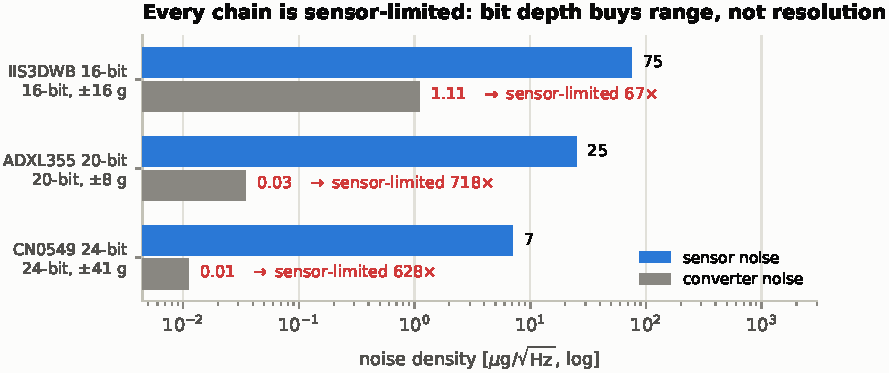
\includegraphics[width=0.80\textwidth]{cn0549_noise_floor.pdf}
  \\[2mm]
  \begin{columns}[T]
    \begin{column}{0.49\textwidth}
      \scriptsize
      The first version of this experiment quantised one record to 16, 20 and
      24 bits and compared the BPFO harmonic ratio. \textbf{All three agreed to
      three decimal places} at every severity from 0.002 to 0.6.
      \\[2mm]
      That was not a bug. Every chain here is sensor-limited by 67--718$\times$:
      adding converter bits to a sensor-limited measurement buys dynamic range,
      not resolution.
    \end{column}
    \begin{column}{0.49\textwidth}
      \scriptsize\color{pdmink2}
      A 16-bit MEMS part's ADC is \emph{not} what limits it. Its own 75
      $\mu$g/$\sqrt{\mathrm{Hz}}$ sensor noise is 67$\times$ above its
      quantisation floor.
      \\[2mm]
      The same arithmetic appears in the agent's start-up report for every
      channel, and is asserted as a test --- if it ever fails, the chain became
      converter-limited and this slide needs rewriting.
    \end{column}
  \end{columns}
\end{frame}

\begin{frame}{And a 10$\times$ quieter sensor did not detect earlier either}
  \centering
  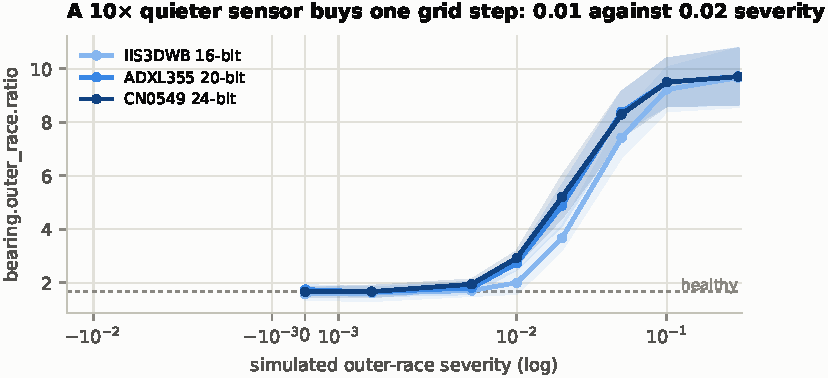
\includegraphics[width=0.76\textwidth]{cn0549_detection.pdf}
  \\[1mm]
  \begin{columns}[T]
    \begin{column}{0.49\textwidth}
      \scriptsize
      All three chains first separate fault from healthy at simulated severity
      \textbf{0.01}. The piezo gives a stronger signature once one exists
      (3.26 against 2.00) --- useful for \emph{severity estimation}, not for
      detection.
      \\[2mm]
      The machine's own broadband noise, not the sensor's, sets the floor.
    \end{column}
    \begin{column}{0.49\textwidth}
      \scriptsize\color{pdmcrit}
      \textbf{So why buy it?} Not resolution.
      \par\color{pdmink2}
      \textbf{Bandwidth:} DC--40 kHz against the IIS3DWB's 6.3 kHz. Lubrication
      distress emits at 20--40 kHz, which no MEMS part here can see
      \emph{at all}. Categorical, not incremental.
      \\[1mm]
      \textbf{Traceability:} when a fleet disagrees with itself, a certificate
      settles it.
      \\[1mm]
      \textbf{DC accuracy:} tilt and thrust are measurements, not
      AC-coupling artefacts.
    \end{column}
  \end{columns}
  \srcnote{Simulator result. The \emph{physics} argument --- sensor noise
  dominates ADC noise by 600$\times$ --- is datasheet arithmetic and stands
  alone; the detection threshold does not. Stage 2 of the validation protocol
  is the experiment that would replace it.}
\end{frame}

% --------------------------------------------- finding 2: the disconnected one --
\begin{frame}{Finding 2: a cut cable is diagnosed as a fault}
  \centering
  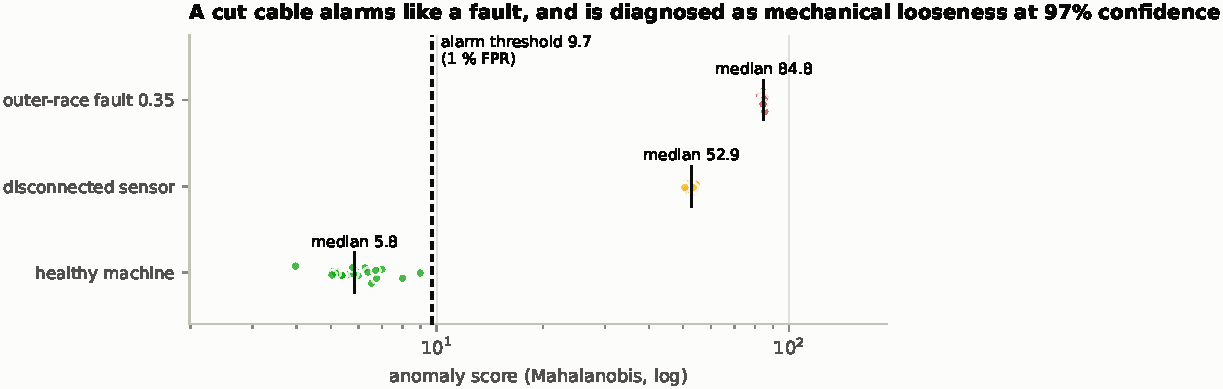
\includegraphics[width=0.84\textwidth]{cn0549_disconnected.pdf}
  \\[2mm]
  \begin{columns}[T]
    \begin{column}{0.49\textwidth}
      \scriptsize
      The prediction was that converter noise --- the smoothest signal the
      system will ever see --- would score \emph{below} healthy, making the
      worst possible condition invisible.
      \\[2mm]
      \textbf{Wrong.} Distance from healthy is not ordered by smoothness:
      converter noise is far outside the healthy manifold, in a different
      direction, and a quadratic-form detector does not care which.
      Featureless is as anomalous as faulty.
    \end{column}
    \begin{column}{0.49\textwidth}
      \scriptsize\color{pdmcrit}
      \textbf{The real failure is a level up.}
      \par\color{pdmink2}
      The detector alarms, and the rule base then diagnoses the noise:
      \textbf{mechanical looseness, 97 \% confidence}.
      \\[1mm]
      A fitter is dispatched to a healthy machine; the real fault is a
      connector; and when the fitter finds nothing, the programme loses
      credibility in the way that ends programmes.
      \\[1mm]
      Unfixable in the data. It needs an out-of-band check.
    \end{column}
  \end{columns}
\end{frame}

% ------------------------------------------------------------------ the check --
\begin{frame}{The out-of-band check: IEPE bias}
  \begin{columns}[T]
    \begin{column}{0.47\textwidth}
      \scriptsize
      An IEPE sensor idles at a known bias on its constant-current supply, so
      the bias voltage \emph{is} the cable's state.
      \\[2mm]
      \begin{tabular}{@{}llr@{}}
        \toprule
        \textbf{Bias} & \textbf{State} & \\
        \midrule
        $\geq$ 85 \% of supply & \texttt{open}   & cut cable \\
        6--16 V                & \texttt{ok}     & live sensor \\
        $\leq$ 1 V             & \texttt{short}  & shorted line \\
        anything else          & \texttt{unknown} & \textcolor{pdmcrit}{not a pass} \\
        \bottomrule
      \end{tabular}
      \\[2mm]
      A pure function of (voltage, supply rail), so the whole decision table is
      tested with no hardware --- which matters, because this is the check that
      catches the failure the data cannot show.
    \end{column}
    \begin{column}{0.47\textwidth}
      \scriptsize
      \textbf{\texttt{open()} refuses to start, it does not warn.}
      \\[1mm]
      The costs are asymmetric. A node that refuses produces a loud, immediate,
      correctly-attributed failure. A node that starts on a cut cable produces
      months of data showing a beautifully smooth machine --- and
      \textbf{nobody questions good news}.
      \\[2mm]
      \texttt{unknown} is not a pass either. That band is where a wrong sensor
      type, an over-long cable and a failing current source live, and
      ``probably fine'' is how the previous slide begins.
      \\[2mm]
      \color{pdmink2}
      Open item: the bias should be \emph{trended}, not just gated. A slowly
      falling bias is a failing source or a wetting connector, visible weeks
      before it trips a threshold.
    \end{column}
  \end{columns}
  \takeaway{The most valuable feature on a EUR 700 instrument is a voltmeter
  reading on its own cable.}
\end{frame}

% -------------------------------------------------------------------- choices --
\begin{frame}{Two configuration choices that silently change the numbers}
  \begin{columns}[T]
    \begin{column}{0.49\textwidth}
      \scriptsize
      \textbf{The anti-alias filter is a choice, not a default.}
      \\[1mm]
      \begin{tabular}{@{}lll@{}}
        \toprule
        & \textbf{Transition} & \textbf{Group delay} \\
        \midrule
        \texttt{sinc5}    & sharp & long \\
        \texttt{wideband} & flat to 0.433$\times$ & short \\
        \bottomrule
      \end{tabular}
      \\[1mm]
      Spectra want sinc5. \textbf{Impacts and envelopes want wideband}, because
      sinc5's long impulse response smears the impacts the envelope detector
      exists to find.
      \\[1mm]
      So \texttt{filter\_type} has no default and the agent prints it at start.
    \end{column}
    \begin{column}{0.49\textwidth}
      \scriptsize
      \textbf{The clip check comes before DC removal.}
      \\[1mm]
      This chain is DC-coupled, so the bias appears as a large offset that must
      be removed before any spectral work --- left in, it leaks out of bin 0
      into the low orders through the window skirts.
      \\[1mm]
      But the converter clips on the \emph{total} signal including the offset.
      Removing it first and then checking would hide exactly the condition
      being looked for: a signal riding a large offset that saturates on one
      side only.
      \\[1mm]
      \color{pdmink2}
      The removed amount is reported, not discarded --- a drifting DC offset
      tracks the current source's health and the sensor's temperature.
    \end{column}
  \end{columns}
\end{frame}

% ------------------------------------------------------------------- verdict ---
\begin{frame}{What is missing, and what it would settle}
  \begin{columns}[T]
    \begin{column}{0.52\textwidth}
      \scriptsize
      \begin{tabular}{@{}ll@{}}
        \toprule
        IEPE bias decision table      & 5 tests \\
        Config + calibration validated& 6 tests \\
        Experiments reproducible      & JSON committed \\
        Shared agent end-to-end       & 36 tests \\
        Sensor-limited claim          & asserted as a test \\
        \midrule
        Run against a CN0549          & \textcolor{pdmcrit}{no} \\
        IIO attribute names verified  & \textcolor{pdmcrit}{no} \\
        Reference-shaker calibration  & \textcolor{pdmcrit}{no} \\
        Cross-validation vs MEMS      & \textcolor{pdmcrit}{no} \\
        20--40 kHz AE band            & \textcolor{pdmcrit}{no} \\
        Calibration certificate       & placeholder \\
        \bottomrule
      \end{tabular}
    \end{column}
    \begin{column}{0.44\textwidth}
      \scriptsize
      \textbf{The highest-value missing experiment in this repository:} mount a
      CN0549 channel and a MEMS node on the \emph{same} bearing housing, run a
      seeded-defect rig, and compare velocity RMS, kurtogram band choice,
      BPFO/BPFI ratios and detection severity.
      \\[2mm]
      That replaces finding 1's simulator result with a real one --- and it is
      the only way to know whether a EUR 90 node's numbers can be trusted.
      \\[2mm]
      \color{pdmink2}
      Second: 20--40 kHz under deliberate lubrication starvation. It is the
      kit's strongest remaining argument and nothing here has measured it.
    \end{column}
  \end{columns}
  \takeaway{A bandwidth-and-traceability purchase wearing a resolution label.
  Buy it to validate a fleet, not to be one.}
\end{frame}

\end{document}
